\documentclass[conference]{IEEEtran}

\usepackage{cite}
\usepackage{amsmath,amssymb,amsfonts}
\usepackage{algorithmic}
\usepackage{graphicx}
\usepackage{textcomp}
\usepackage{xcolor}
\usepackage{csquotes}

\def\BibTeX{{\rm B\kern-.05em{\sc i\kern-.025em b}\kern-.08em
  T\kern-.1667em\lower.7ex\hbox{E}\kern-.125emX}}
\begin{document}

\title{Decentralized Access Control}%*\\

\author{
  \IEEEauthorblockN{Heinrich Lorenz}
  Karlsruhe, Germany \\
  lorenz.heinrich@student.kit.edu
}

\maketitle

\begin{abstract}
  Lorem ipsum dolor sit amet, consectetur adipiscing elit. sed non risus. Suspendisse lectus tortor, dignissim sit amet, adipiscing nec, ultricies sed, dolor. Cras elementum ultrices diam.
\end{abstract}

\begin{IEEEkeywords}
  lorem, ipsum, dolor, sit, amet
\end{IEEEkeywords}

\section{Introduction}
The applications of shared personal data cannot be denied.
Patients may want as much data for their diagnosis to be used as possible while also wanting their medical records to be available for others. \cite{hollis_share_2016}
Athletes may want to share fitness data with service providers for analysis, and users of the web may want their data to be used for a personalized experience.\cite{nasir_council_nodate}
However, if individuals do not want to publicly share their data, some kind of mechanism is required allowing them to specify \textit{who} gets access to \textit{what} data \textit{when}.

Current industry standards rely on centralized authorization and authentication mechanisms acting on behalf of a user to manage data access. \cite{hardt_oauth_2012,noauthor_googles_nodate}
These practices demand individuals to trust in the correctness of these services while most of the time no effort is made to provide insight into the actual processes.
Additionally, due to the assumption that the service providers are a part of the user's trusted domain, the data is often visible in clear to them, leading to increasing privacy concerns.
This situation has led to emerging voices questioning who should wield ultimate power over data and how the users' ability to manage their data without relying on third parties can be enhanced. \cite{noauthor_w3f_nodate}
In essence, this describes the idea of data sovereignty where self-sovereign individuals with the ability to manage their identity and data without trusted intermediates can interact and share data while preserving their privacy. \cite{ernstberger_sok_2023}

In this work, the status quo of access control systems currently used in web-based services will be analyzed while also formulating the key aspects of an access control system.
After clarifying the shortcomings current practices suffer from, an alternative model based on decentralized technologies will be introduced.
By the example of the decentralized access control system Droplet, concrete aspects of decentralized access control will be discussed in further detail, concluding with an evaluation of the contributions of decentralized access control to the idea of data sovereignty.

\section{Access Control}
In the context of web services, the term \textit{access control} refers to \enquote{the process of granting or denying specific requests to [\dots] obtain and use information and related information processing services [\dots]}. [reference] % // TODO: add a citation
Traditionally, in the realm of access control, an individual who owns the data subject to access control is designated as the \textit{resource owner}, while the entity seeking access is commonly referred to as the \textit{client}.
Moreover, the infrastructure housing the protected resources is denoted as the \textit{resource server}.

\subsection{Access Control in Web 2.0}
A web service (client) requesting access to an access-restricted resource hosted on a resource server can access the resource by using the resource owner's credentials.
Using this method to grant access comes with several issues.
First, the resource owner has no option but the update his credentials if he wants to revoke the granted access.
Second, by disclosing the credentials to the resource server, the client gets access to all resources hosted on that server and third, the compromisation of that client results in a compromisation of the resource owner's credentials and therefore all of the resources of the user hosted on the resource server.
Analyzing these issues, one can conclude that the desirable properties of an access control system include

%//TODO: maybe inline?
\begin{enumerate}
  \item \textbf{Fine-Grained Access Scope:} Resource owners should be able to specify to which resources they grant access at what point in time.
  \item \textbf{Individual Access:} Resource owners should be able to independently grant access to different clients.
  \item \textbf{Revocability of Access:} Resource owners should be able to revoke granted access at any time with minimal effort.
\end{enumerate}

%//TODO: maybe suits better as an introduction
Web 2.0, as we know it today, heavily relies on contributing, creating, and collaborating on various platforms. \cite{community_web_2019}
As a consequence, there is a demand for systems supporting fine-grained access control to the resources generated and owned by users. 
To address the challenges the above-described naive authorization approach entails, the OAuth protocol delineates an authorization flow for access control systems outlining the process by which clients can request access to protected resources while enabling resource owners to fulfill these requests without disclosing their credentials.

\subsubsection*{OAuth}
The protocol introduces an \textit{authorization server} that authenticates clients and enforces restricted access to resources on behalf of the resource owner.
The client can request access to a resource of the resource owner and by that obtain an \textit{authorization grant}.
This grant declares the client as authorized by the resource owner and enables the client to obtain an \textit{access token} from the authorization server in exchange for the authorization grant.
This token contains a set of attributes specifying to which resource the client has access to.
Using this token, the client can request the resource from the resource server, which in turn validates the access token and returns the resource in case of a valid token. \cite{hardt_oauth_2012}

\subsection{Shortcomings of Centralized Access Control}
Access control systems based on the OAuth 2.0 framework indeed mitigate the problems introduced by the naive authorization method by separating the resource owner from the client.
The protocol allows the resource owner the individually specify which client gets access to what data when enforced by the access tokens issued by the authorization server. \cite{hardt_oauth_2012}
Thereby key aspects of an access control system are implemented including the properties defined above.

However, the centralized nature of the authorization and resource server introduces a new dimension of concerns.
Users must trust these entities to comply with the OAuth specification and effectively protect their data by prohibiting access to data from unauthorized clients.
Additionally, since the OAuth protocol builds upon trust in centralized entities, data on the resource server is not protected from the service providers violating the privacy of users and increasing the risk of data breaches.
Centralized access control systems also suffer from a single point of failure increasing the risk of unauthorized access.

Unfortunately, these concerns are not only valid in theory but regard the everyday experience of individuals using these services.
Chen, 2014 examined popular mobile apps using OAuth 2.0 and found that more than half of the examined applications implemented the OAuth 2.0 flow incorrectly, thus making the application, and consequently the data of the users vulnerable. \cite{chen_oauth_2014}

\section{Decentralized Access Control}
With the upcoming popularity of IoT devices especially in the realm of wearables and sensors on and around humans, highly privacy-relevant data is generated on a large scale. \cite{zhang_cloud_2015}
Data-centric centralized industry practices assume that the service provider is part of the user's trusted domain and therefore no effort is made to ensure data confidentiality, allowing for uncontrolled sharing of this highly personal data. \cite{shafagh_droplet_2020}
These industry practices have led to attempts to control data privacy via privacy regulations that introduced the challenge of ensuring that service providers follow accordingly. \cite{noauthor_general_nodate}

Shortcomings in privacy have led to a call for a paradigm shift towards a user-centric approach, as opposed to a data-centric approach, both in technical and non-technical communities. \cite{ernstberger_sok_2023, shafagh_droplet_2020}

\subsubsection{Definition}
Decentralized Access Control enables data owners to verifiably share data with data consumers by specifying fine-grained access policies without exposing the data in clear to any third party and without the need to rely on any trusted intermediate.
The primary goal of the concept of decentralized access control is to bring back the power over the data to the data owners by treating data privacy as a first-class citizen. \cite{ernstberger_sok_2023}

The primary goal of the concept of decentralized access control is to bring back the power over the data to the data owners by treating data privacy as a first-class citizen.

\subsubsection{Model}

The model of decentralized access control is described as follows:

\begin{itemize}
  \item \textbf{Data Owner:} A User that wants to share personal data with a data consumer.
  \item \textbf{Data Consumer:} A service that wants to access personal data of the user.
  \item \textbf{Storage:} The location where the encrypted data units are stored.
  The Storage can be local, a centralized, or a decentralized storage provider.
  \item \textbf{Access Controler:} Computational Nodes, granting access to a ciphertext by releasing the according secret shares to the requesting data consumer after validation of the proof of policy satisfaction provided by the data consumer.
  \item \textbf{Access Policies:} Policies specified by the user describing under which conditions a data consumer can access the secret shares of a specific ciphertext.
  \item \textbf{Distributed Ledger:} A technology maintaining a globally verifiable, append-only distributed log of transactions. A popular example is the blockchain technology. 
\end{itemize}

\begin{figure}[htbp]
  \centering
  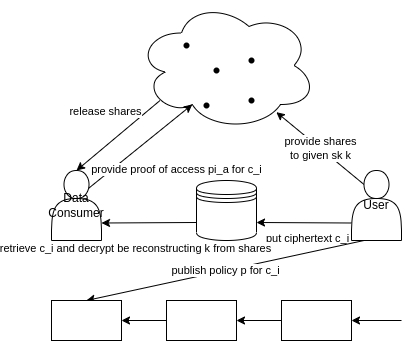
\includegraphics[width=0.4\textwidth]{figures/decentralized_access_control.png}
  \caption{Decentralized Access Control}
  \label{fig:decentralized_access_control}
\end{figure}
Fig. \ref{fig:decentralized_access_control} illustrates the steps required to share user data with a data consumer using the decentralized access control model.

For a given secret k, she computes a set of shares that gets sent to a committee of access controllers.

Using this secret k for a data item that is desirable to grant access to, the data item is encrypted and stored in the user's wallet or another storage system, and an access policy is published on-chain specifying under which conditions a data consumer is authorized to access the data item.

A data consumer wishing to access the data item is required to supply proof to the committee of access controller stating that the data consumer fulfills the access policy.

After validating the supplied proof from the data consumer the committee of access controllers releases the secret shares of the secret key k that was used for the encryption of the data item, the data consumer proved to have access to.

Using the shares and the ciphertext of the data item, the data consumer can successfully decipher it by reconstructing the secret k.

An Update to the access policy only requires the user to publish a new access policy to the distributed ledger.

\subsubsection{Additional Properties}
\begin{itemize}
  \item Data confidentiality
  \item Anonymity
  \item Auditability
  \item Policy Confidentiality
  \item Fair Access
  \item Access Revocation
\end{itemize}

\subsection{Decentralized Access Control with the Example of Calypso}

\section{Confidential yet Expressive Access Policies?}

\subsection{On-Chain Secrets}


\bibliographystyle{IEEEtran}
\bibliography{references}

\end{document}
